\documentclass{beamer}
% \usepackage{graphicx}
% \usepackage[all,cmtip]{xy}
\usepackage{tikz}
\usepackage{tikz-cd}
\usepackage{qtree}
\usepackage{stmaryrd}
% \usepackage{diagxy}
\usepackage{amsfonts}
\usepackage{amssymb}
\usepackage{amsmath}
\usepackage{amscd}
\usepackage{amsthm}
\usepackage{bbm}
%\usepackage{pictexwd,dcpic}
% \usepackage[mathcal]{euscript}
\usepackage[utf8]{inputenc}
%\usepackage[T1]{fontenc}
\usepackage{lmodern}
%\usepackage{setspace}
%\usepackage{mathpartir}
% \usepackage{proof}
%\setstretch{1}
\title{Theoretical Equivalence and Invariant Structure}
\author{Hans Halvorson}
\date{May 18, 2013}
\usetheme{Singapore}
\begin{document}
\def\2{\mathcal}
\def\7{\mathbb}
\begin{frame}

% Keywords: verbal disputes, synonymous theories

\maketitle

\end{frame}

\begin{frame}

\begin{itemize}
\item If $T_1$ and $T_2$ are equivalent, then what must they share in
  common?  What are the ``invariants'' of theoretical equivalence?
\item What is preserved in theory change?  What are the ``invariants''
  of theory change?
\item What parts of our current theories ought we to believe?
\end{itemize}
\end{frame}

\begin{frame}{Purported theoretical equivalences}

\begin{tabular}{rcll}
Schr\"odinger & $\cong$ & Heisenberg & (von Neumann) \\ \\ 
Lagrangian & $\cong$ & Hamiltonian & (Legendre) \\ \\ 
Newtonian Gravity & $\cong$ &   Newton-Cartan Gravity & (Weatherall) \\ \\ 
Spacetimes & $\cong$ & Leibniz Algebras \\ \\ 
Geometry of Points & $\cong$ & Geometry of Lines \\ \\ 
Mereological Nihilism & $\cong$ & Compositionalism & (Hirsch) \\ \\ 
Relativism & $\cong$ & Expressivism & (Dreier) \end{tabular}

\end{frame}


\begin{frame}{Naive accounts of equivalence}

\begin{itemize}
\item $T_1$ and $T_2$ are equivalent just in case they say the same
  thing, i.e.\ they have the same content.
\begin{itemize}
\item Correct but uninformative.  How to specify content?
\end{itemize}
\end{itemize}

\begin{itemize}
\item $T_1$ and $T_2$ are equivalent just in case they make the same
  predictions.
\end{itemize}


\begin{itemize}
\item $T_1$ and $T_2$ are equivalent just in case they are true in
  exactly the same possible worlds.
\end{itemize}

\begin{itemize}
\item $T_1$ and $T_2$ are equivalent just in case they have the same
  set of models.
\end{itemize}
\end{frame}

\begin{frame}

  \begin{quote} ``Theories are extralinguistic entities which may be
    described or characterized by a number of different linguistic
    formulations.'' Suppe 1977 \end{quote}

  \begin{quote} ``While a theory may have many different formulations,
    its set of models is what is important.''  van Fraassen
    2008 \end{quote}

\begin{tikzcd}[ampersand replacement=\&]
T_1 \arrow{dr} \& \& T_2 \arrow{dl} \\
\& \2M \end{tikzcd} 


\end{frame}


\begin{frame}{Spectrum of equivalence}

  \begin{tikzpicture}[scale=0.9]
\tikzstyle{every node}=[font=\tiny]
\draw [<-> ,thick ] (0,0) -- (10,0);
\node[align=center, below] at (0,2.5) {same string \\ of symbols};
\node[align=center, below] at (1.5,1.5) {same language};
\node[align=center, below] at (1.5,3) {same axioms};
\node[align=center, below] at (5.5,2.5) {theoretical \\ equivalence?};
\node[align=center, below] at (8,2.5) {empirical \\ equivalence};
\node[align=center, below] at (0,-0.25) {finer};
\node[align=center, below] at (10,-0.25) {coarser};
\node[align=center, below] at (10,2.5) {consistent? \\ (Putnam)};
\node[align=center, below] at (0,-1.5) {everybody  \\ disagrees};
\node[align=center, below] at (10,-1.5) {nobody \\ disagrees};
\end{tikzpicture}

%% all theories say the same thing; 


\end{frame}





\begin{frame}{Definitional equivalence}


\begin{itemize}
\item Empirical equivalence was a suitable notion for
  verificationists, circa 1920--1950.
\item The idea of \textcolor{blue}{definitionally equivalent} or
  \textcolor{blue}{synonymous} theories due to Tarski or Montague,
  circa 1960.
\item Co-opted for philosophy of science by Glymour: ``Theoretical
  realism and theoretical equivalence'' 1970.
\end{itemize}

\end{frame}

\begin{frame}{Definitional equivalence}

\begin{tabular}{llllll}
 & & $T_1$  & & $T_2$ \\ \\ 
\hline \hline \\
Language &  & $\{ c \}$ & & $\{ P \}$ \\ \\
Axioms   &  & $\emptyset$ & & $\exists !xPx$ \end{tabular}

% Interesting feature: Although the theories are equivalent, language
% 2 might be considered preferable, because it gives the option of
% denying existence of a $P$.  Compare with the Quine "pegasizing"
% maneuver

% Could you have reason to choose theory 2 over theory 1?  Yes,
% indicates Quine


\end{frame}  

\begin{frame}{Definitional equivalence}

\begin{tabular}{llllll}
  & & $T_1$  & & $T_2$ \\ \\ 
  \hline \hline \\
  Language &  & $\{ \circ ,-1,e \}$ & & $\{ \circ ,e \}$ \\ \\
  Axioms   &  & associativity & & associativity   \\  
  &  & $e$ is an identity & & $e$ is an identity \\ 
  &  & $x\circ x^{-1}=e=x^{-1}\circ x$ & & $\exists !y(x\circ
  y = e = y\circ x)$ 
\end{tabular} 
\end{frame}

\begin{frame}{Interpretations and model maps}

  \begin{definition} An \textcolor{green}{interpretation} or
    \textcolor{green}{translation} of $T_1$ into $T_2$ consists of a
    map $F$ that takes $n$-place relation symbols of $L_1$ to
    $n$-place open formulas of $L_2$, and such that:
$$ T_1\vdash \phi \qquad \Longrightarrow \qquad T_2\vdash \phi
^F $$ \end{definition}

\bigskip

\begin{tabular}{ccc} \begin{tikzcd}[ampersand replacement=\&]
T_1 \arrow{d}{F} \\ 
T_2   \end{tikzcd} & & 
\begin{tikzcd}[ampersand replacement=\&] \2M _1  \\
  \2M _2 \arrow[swap]{u}{F^*} \end{tikzcd} \end{tabular}

\end{frame}

\begin{frame}{Definitional extension}

\begin{definition}
  $T'$ is a \textcolor{green}{definitional extension} of $T$ if:
\begin{itemize}
\item $T'$ explicitly defines each predicate symbol $R$ of $L'$ in
  terms of the language $L$:
$$ T'\quad \models\quad \forall x(R(x)\leftrightarrow \phi _R(x)) $$
\item $T'$ is a conservative extension of $T$.
\end{itemize}
\end{definition}

\end{frame}

\begin{frame}{Definitional extension}

\begin{tabular}{ccc}
\begin{tikzcd}[ampersand replacement=\&]
T' \arrow[transform canvas={xshift=1ex}]{d}{P}  \\
T   \arrow[transform canvas={xshift=-1ex}]{u}{I} \end{tikzcd}
& & 
\begin{tikzcd}[ampersand replacement=\&]
\2M ' \arrow[transform canvas={xshift=-1ex},swap]{d}{I^*} \\
\2M \arrow[transform canvas={xshift=1ex},swap]{u}{P^*}
\end{tikzcd}
\end{tabular}


\begin{itemize}
\item $T$ and $T'$ are mutually interpretable.
\item For each sentence $\phi$ of $L'$
$$ T' \: \models \: (IP\phi )\leftrightarrow \phi $$
\item For each sentence $\psi$ of $L$
$$ T \: \models \: (PI\psi )\leftrightarrow \psi $$
\item The category of models of $T$ is isomorphic to the category of
  models of $T'$.
\end{itemize}

\end{frame}


\begin{frame}{Common definitional extension}

\begin{definition}
Two theories $T_1$ and $T_2$ are \textcolor{green}{definitionally equivalent} just
in case they have a common definitional extension. \end{definition}


\begin{tabular}{cc}
\begin{tikzcd}[ampersand replacement=\&]
\& T' \arrow[transform canvas={xshift=-1ex},swap]{dl}{P_1} \arrow[transform canvas={xshift=1ex}]{dr}{P_2} \& \\
T_1 \arrow[transform canvas={xshift=1ex},swap]{ur}{I_1} \arrow[dashed,swap]{rr}  \& \& T_2 \arrow[transform canvas={xshift=-1ex}]{ul}{I_2} \end{tikzcd}
& 
\begin{tikzcd}[ampersand replacement=\&]
\& \2M ' \arrow{dr} \arrow{dl} \& \\
\2M _1 \arrow[transform canvas={yshift=0.5ex},dashed]{rr}{\mathcal{F}} \&
\& \2M _2 \arrow[transform canvas={yshift=-0.5ex},dashed]{ll}{\mathcal{G}} \end{tikzcd} \end{tabular}


\end{frame}


\begin{frame}{Invariants of definitional equivalence}

\tikzstyle{vecArrow} = [thick, decoration={markings,mark=at position
   1 with {\arrow[semithick]{open triangle 60}}},
   double distance=1.4pt, shorten >= 5.5pt,
   preaction = {decorate},
   postaction = {draw,line width=1.4pt, white,shorten >= 4.5pt}]
\tikzstyle{innerWhite} = [semithick, white,line width=1.4pt, shorten >= 4.5pt]

\tikzset{every loop/.style={min
    distance=10mm,in=60,out=120,looseness=2}}

\tikzset{
doublearrow/.style={draw, double distance=4pt, ->}
}

\begin{tikzpicture}

\draw[line width=0.25mm,double, double distance=0.7mm] (1.5,2.5) -- (0.75,1.5);

\draw[line width=0.25mm,double, double distance=0.7mm] (3.5,2.5) -- (4.5,1.5);


\draw (2.5,4) ellipse (2cm and 1.5cm);
\draw (0,0) ellipse (2cm and 1.5cm);
\draw (5.5,0) ellipse (2cm and 1.5cm);

\node[align=center, below] at (-1,2)%
{$\2M _1$};
\node[align=center, below] at (6.5,2)%
{$\2M _2$};
\node[align=center, below] at (4.25,5.75)%
{$\2M _0$};

\node (A) at (0,0) {};
\draw[fill] (0,0) circle [radius=0.05];
\node (B) at (-0.7,0.7) {};
\draw[fill] (-0.7,0.7) circle [radius=0.05];
\node (C) at (1,-0.1) {};
\draw[fill] (1,-0.1) circle [radius=0.05];
\draw [->] (A) to [bend right=30] (B);
\path [->] (C) edge[loop above] node[left=1pt] {} (C);

\node (X) at (5.5,0) {};
\draw[fill] (5.5,0) circle [radius=0.05];
\node (Y) at (4.8,0.7) {};
\draw[fill] (4.8,0.7) circle [radius=0.05];
\node (Z) at (6.5,-0.1) {};
\draw[fill] (6.5,-0.1) circle [radius=0.05];
\draw [->] (X) to [bend right=30] (Y);
\path [->] (Z) edge[loop above] node[left=1pt] {} (Z);

\node (D) at (2.5,4) {};
\draw[fill] (2.5,4) circle [radius=0.05];
\node (E) at (1.8,4.7) {};
\draw[fill] (1.8,4.7) circle [radius=0.05];
\node (F) at (3.5,3.9) {};
\draw[fill] (3.5,3.9) circle [radius=0.05];
\draw [->] (D) to [bend right=30] (E);
\path [->] (F) edge[loop above] node[left=1pt] {} (F);


% \draw[fill] (0.7,0.2) circle [radius=0.05];
% \draw[->] (0.7,0.2) arc [start angle=-190, end angle=150, x radius=0.25cm, y radius=0.25cm];
% \draw[fill] (0,-0.5) circle [radius=0.05];
% \draw[fill] (-1,0.5) circle [radius=0.05];
% \draw [->] (-0.05,-0.35) arc [radius=1.4, start angle=20, end angle= 70];
% % \draw[->] (-0.1,-0.4) -- (-0.9,0.4);

% \draw[fill] (6,0.5) circle [radius=0.05];
% \draw[fill] (5.5,-0.2) circle [radius=0.05];
% \draw[fill] (4.8,0.2) circle [radius=0.05];
\end{tikzpicture}


\end{frame}


\begin{frame}{These models describe the same world}

% internal picture of models

\begin{tikzpicture}
\draw (2.5,4) ellipse (1.5cm and 1.5cm);
\draw (0,0) ellipse (1.5cm and 1.5cm);
\draw (5,0) ellipse (1.5cm and 1.5cm);

\node[align=center, below] at (3,6)%
{$A$};
\node[align=center, below] at (-1,2)%
{$A|_{\2L _1}$};
\node[align=center, below] at (6,2)%
{$A|_{\2L _2}$};


\filldraw[fill opacity=0.25,fill=green] (0.25,0.25) ellipse (0.35cm and 0.35cm);
\node[align=center, below] at (0.25,1.2)%
{\small $[\phi (x)]$};

% right 2.5 up 4
\filldraw[fill opacity=0.25,fill=green] (2.75,4.25) ellipse (0.35cm and 0.35cm);
\node[align=center, below] at (2.75,5.2)%
{\small $[\phi (x)]$};

% right 5
\filldraw[fill opacity=0.25,fill=green] (5.25,0.25) ellipse (0.35cm and 0.35cm);
\node[align=center, below] at (5.25,1.2)%
{\small $[\psi (x)]$};



\end{tikzpicture}

\end{frame}

\begin{frame}


\begin{itemize}
\item $\2F :\2M _1\to\2M _2$ is an equivalence of categories.
\item $\2F (A)$ and $A$ are \emph{isomorphic}
\begin{itemize}
\item have the same symmetry groups;
\item domains have same cardinality;
\item same definable sets.
\end{itemize}
\end{itemize}

\end{frame}

\begin{frame}{Cutting nature at its joints}

  \textbf{Model Isomorphism Criterion:} If two theories are equivalent
  then their models are pairwise isomorphic.

\bigskip
\begin{itemize}
\item Hamiltonian mechanics and Lagrangian mechanics are
  \textcolor{red}{not} equivalent.
\item Spacetime theories and Leibniz algebra theories are
  \textcolor{red}{not} equivalent.
\end{itemize}
\bigskip

\textbf{Structural Realism:} A theory is true if the WORLD is
  isomorphic to one of its models.

\end{frame}

\begin{frame}

\begin{figure}[!h]
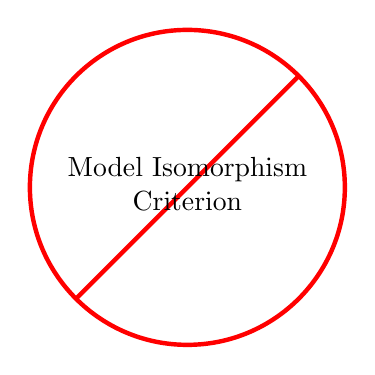
\begin{tikzpicture}
\draw[color=red,ultra thick] (0,0) ellipse (2cm and 2cm);
\draw[color=red,ultra thick] (-1.42,-1.42) -- (1.42,1.42);
\node[align=center, below] at (0,0.5) {Model Isomorphism \\ Criterion};
\end{tikzpicture}
\end{figure}


\end{frame}


\begin{frame}{Against the model isomorphism criterion}

% T1: sets
% T2: sets of pairs, with designated element of each pair

%% complex numbers as pairs of real numbers  [could we use roots of
%% unity?]
%% T_1 \forall x (x^n = 1)

%% T_2 x,y : 

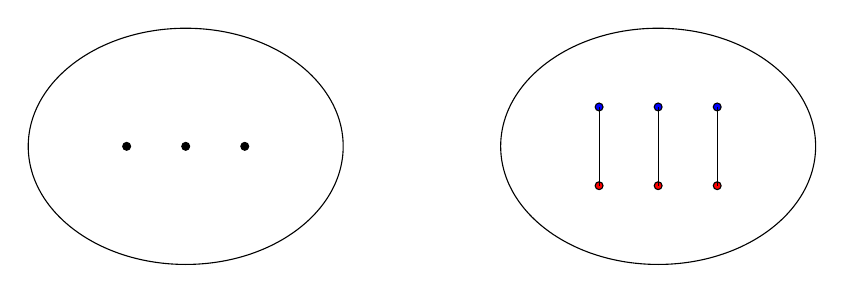
\begin{tikzpicture}
% first model -- set with three elements
\draw (0,0) ellipse (2cm and 1.5cm);
\draw[fill] (-0.75,0) circle [radius=0.05];
\draw[fill] (0,0) circle [radius=0.05];
\draw[fill] (0.75,0) circle [radius=0.05];


% second model -- set with six elements
\draw (6,0) ellipse (2cm and 1.5cm);

\filldraw[fill=red] (5.25,-0.5) circle [radius=0.05];
\draw[fill=red] (6,-0.5) circle [radius=0.05];
\draw[fill=red] (6.75,-0.5) circle [radius=0.05];

\draw[fill=blue] (5.25,0.5) circle [radius=0.05];
\draw[fill=blue] (6,0.5) circle [radius=0.05];
\draw[fill=blue] (6.75,0.5) circle [radius=0.05];

\draw (5.25,-0.5) -- (5.25,0.5);
\draw (6,-0.5) -- (6,0.5);
\draw (6.75,-0.5) -- (6.75,0.5);

\end{tikzpicture}

\end{frame}

%% complex and real numbers

%% Tarski on geometry of points and lines 


\begin{frame}{Against the model isomorphism criterion}

\begin{tikzpicture}[scale=0.7]
    \begin{scope}[thick,font=\scriptsize]
    % Axes:
    % Are simply drawn using line with the `->` option to make them arrows:
    % The main labels of the axes can be places using `node`s:
    \draw [->] (-5,0) -- (5,0) node [above left]  {$\Re\{z\}$};
    \draw [->] (0,-5) -- (0,5) node [below right] {$\Im\{z\}$};

    % Axes labels:
    % Are drawn using small lines and labeled with `node`s. The placement can be set using options
    \iffalse% Single
    % If you only want a single label per axis side:
    \draw (1,-3pt) -- (1,3pt)   node [above] {$1$};
    \draw (-1,-3pt) -- (-1,3pt) node [above] {$-1$};
    \draw (-3pt,1) -- (3pt,1)   node [right] {$i$};
    \draw (-3pt,-1) -- (3pt,-1) node [right] {$-i$};
    \else% Multiple
    % If you want labels at every unit step:
    \foreach \n in {-4,...,-1,1,2,...,3}{%
        \draw (\n,-3pt) -- (\n,3pt)   node [above] {$\n$};
        \draw (-3pt,\n) -- (3pt,\n)   node [right] {$\n i$};
    }
    \fi
    \end{scope}
\node at (5,5) {%
\begin{minipage}{0.3\textwidth}
\begin{eqnarray} c &\longmapsto &\langle
    \mathrm{Re}(c),\mathrm{Im}(c)\rangle \nonumber \\
 r+is &\longmapsfrom & \langle r,s\rangle \nonumber \end{eqnarray} 
\end{minipage} };
\end{tikzpicture}


\end{frame}


\begin{frame}{Against the model isomorphism criterion}

\begin{itemize}
\item A theory already implicitly quantifies over $n$-tuples: $$\exists x_1\exists
  x_2\cdots \exists x_n\phi (x_1,\dots ,x_n)$$
\item Tarski, Szczerba: we must recognize equivalence of geometries
  with \emph{points} as primitives and geometries with \emph{lines} as primitives
\end{itemize}



\end{frame}

\begin{frame}{Multi-sorted logic}

\begin{itemize}
\item Begin with a collection $A,B,C,\dots $ of sorts.
\item Each symbol (relations, functions, variables) of $\2L$ is
  required to be coded by sorts.  example $R:A,A,B$
\item Quantifiers only range over particular sorts.
\item Equality is sort-relative: $=_A$
\item An $\2L$ structure assigns a set/domain/universe to each sort.
\end{itemize}


\end{frame}


\begin{frame}{Defining new universes}

%% adding products

Product sorts (products): The formula $(x_1=x_1)\wedge \cdots \wedge
(x_n=x_n)$ defines a product sort $S_1\times \cdots \times S_n$

\bigskip Reduced sorts (subobjects): A formula $\phi (\overline{x})$
of $L$ defines a reduction of the sort $S_1\times \cdots \times S_n$.

\bigskip \textcolor{green}{Proposal:} $T^+$ should be considered a
definitional extension of $T$.


% % complex numbers in the real numbers

% % example I concocted a couple of weeks ago -- two sorted but

% \begin{tabular}{cccccc}
%   & $T_1$ & & $T_2$ & & $T_3$ \\ \\
%   Language &  sort $A$ & & sorts $A,B$ & & sorts $A,B$ \\ \\ 
%   Axioms   & $\exists _{=2}x:A$ & & $\exists _{=2}x:A$ & & $\exists
%   _{=2}x:A$ \\
%            &                      & & $\exists _{=1}y:B$ \end{tabular} 


\end{frame}

\begin{frame}{Defining new universes}

%% Could use David Marker description

  Suppose that the formula $\phi (x,y)$ defines an equivalence
  relation in~$T$.  Let $T^{eq}$ be the theory that adds a new sort
  $E$, function symbol $f:A;E$, and axioms
  \[ \begin{aligned}
& \forall x^A\forall y^A(\phi (x,y)\leftrightarrow f(x)=f(y)) \\
& \forall z^E\exists x^A(f(x)=z) \end{aligned} \]

\textcolor{green}{Proposal:} $T^{eq}$ should be considered a
definitional extension of $T$.

\end{frame}


\begin{frame}{Morita equivalence}

\textbf{The Hard Way:} Each theory $T$ has a classifying topos $\2E
[T]$.  $T_1$ is Morita equivalent to $T_2$ just in case $\2E [T_1]$
and $\2E [T_2]$ are equivalent toposes.

\bigskip \textbf{The Easy Way:} Theories $T_1$ and $T_2$ are Morita
equivalent just in case they have a common definitional extension ---
in the extended sense where new sorts are definable from old.

\end{frame}

\begin{frame}{Logical accounts of equivalence}

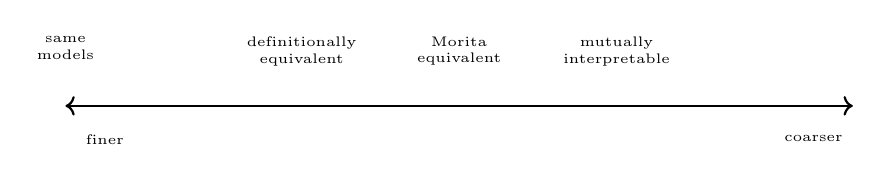
\begin{tikzpicture}
\tikzstyle{every node}=[font=\tiny]
\draw [<-> ,thick ] (0,0) -- (10,0);
\node[align=center, below] at (0,1) {same \\ models};
\node[align=center, below] at (3,1) {definitionally \\ equivalent};
\node[align=center, below] at (7,1) {mutually \\ interpretable};
\node[align=center, below] at (0.5,-0.25) {finer};
\node[align=center, below] at (9.5,-0.25) {coarser};
\node[align=center, below] at (5,1) {Morita \\
  equivalent};
\end{tikzpicture}

\end{frame}

\begin{frame}{Invariants}

\begin{description}
\item[Morita equivalence:] equivalent categories of models
\item[Definitional equivalence:] cardinalities of individual models,
  definable subsets
\end{description}


\bigskip \textbf{Note:} ``Equivalent categories of models'' is
necessary but not sufficient for theoretical equivalence. \newline
\begin{description}
\item[Example:] $X$ versus $X\cup \{ \ast \}$. \end{description}

\end{frame}

\begin{frame}{The case for Morita equivalence}

\begin{itemize}
\item Argument by squeezing: Mathematical examples suggest that other
  criteria are too fine.
\item Argument from mathematical convergence: It's a natural notion,
  both in logic and in category theory.
\item Realizes Putnam's dream of sophisticated realism.  (He himself
  abandoned hope!)
\end{itemize}

\end{frame}


\begin{frame}{Concluding unscientific proposal}

  \textcolor{green}{Proposal:} If $T_1\cong T_2$, then one should
  commit only to the invariants, i.e.\ features on which $T_1$ and
  $T_2$ agree.

  \bigskip \textcolor{red}{Problem:} The models of $T_1$ and $T_2$
  might not agree on anything interesting.

  \bigskip \textcolor{yellow}{Prospect:} There is a more nuanced way
  in which the models describe the same world.




\end{frame}


\end{document}


\smallskip
\begin{quote} 
  ``There is a cow in the barn.'' \\
  ``Let Bessie be one of the cows in the barn.''
\end{quote}

\begin{quote} %  Quine predicate functors
``Pegasus does not exist.'' \\
``The thing that pegasizes does not exist.'' \end{quote}
